\subsection{Эксперименты и наблюдения(параметры)}

\subsubsection{СС(G) тест}

Для начала убедимся в утверждении выдвинутым ранее: Что $CC(G) \rightarrow 0$ при $n \rightarrow \infty$:
Взглянем на график случайного графа по модели Erdős–Rényi со средней степенью вершины 5,
с увеличивающейся выборкой:

\begin{figure}[H]
    \centering
    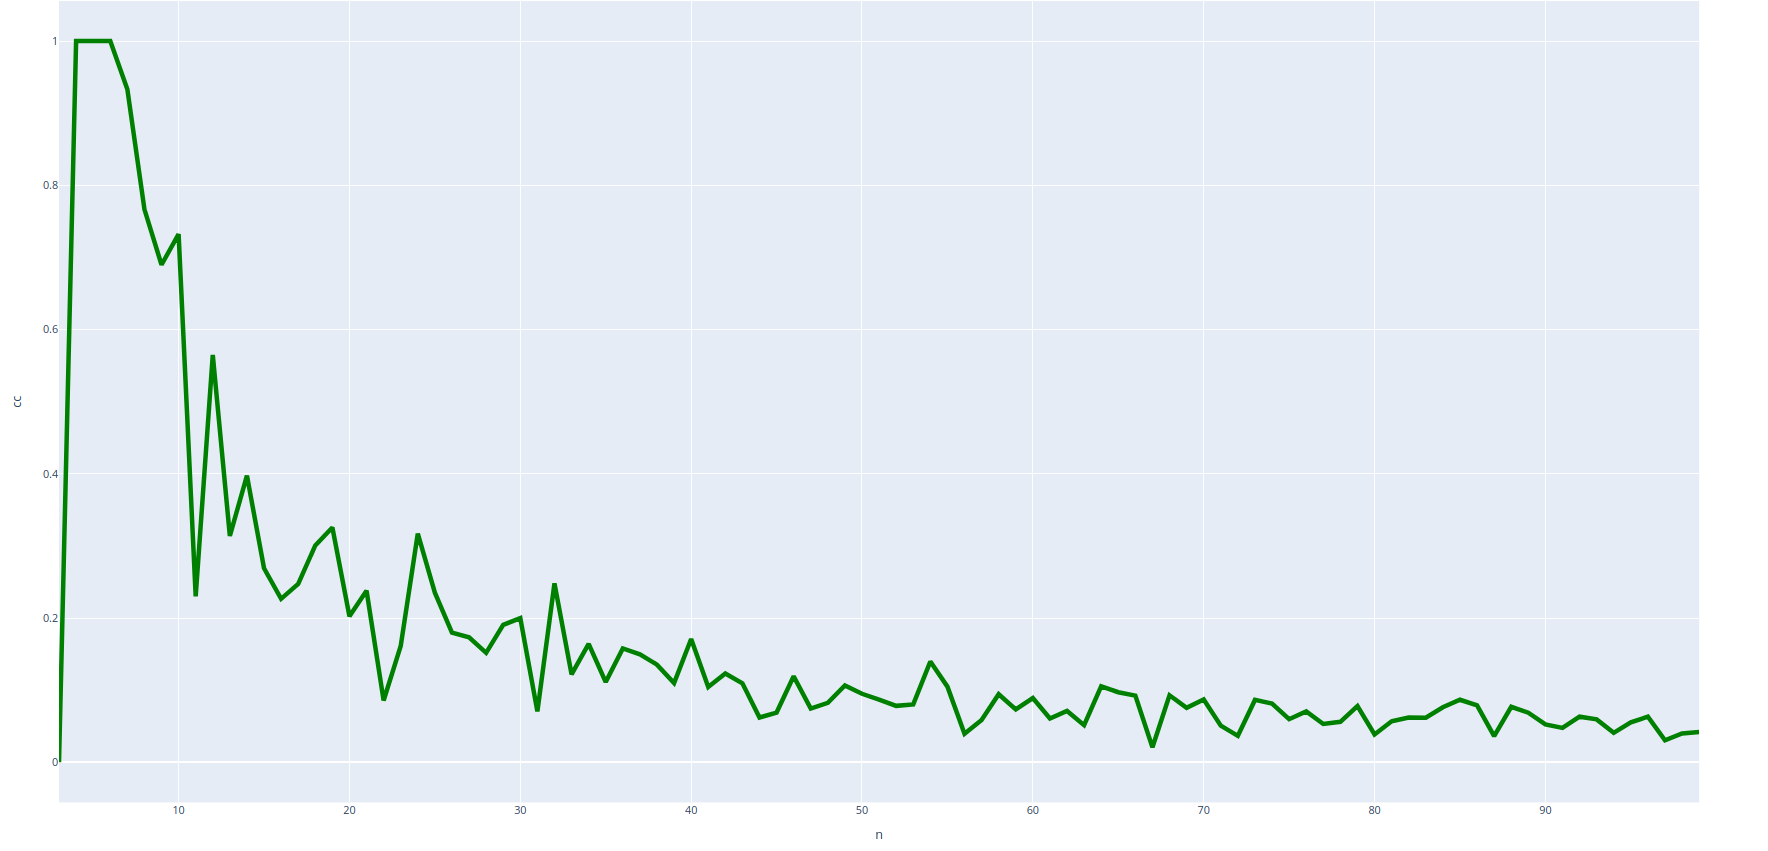
\includegraphics[scale=0.25]{./pictures/random_cc_long_period.png}
    \caption{Зависимость СС(RandomGraph) с ростом выборки} \label{сс от степени вершин}
\end{figure}
Можем наблюдать стабильный нисходящий тренд.

Теперь рассмотрим зависимость коэффицента класстеризации от степени вершин.
В данном примере моя модель содержит 3000 вершин, координаты каждой генерируются случайно 
в диапазона от 0 до 200. Чтобы сравнение было корректным, мне пришлось подобрать параметры
каждого графа, чтобы степени их вершин примерно совпадали.

\begin{figure}[H]
    \centering
    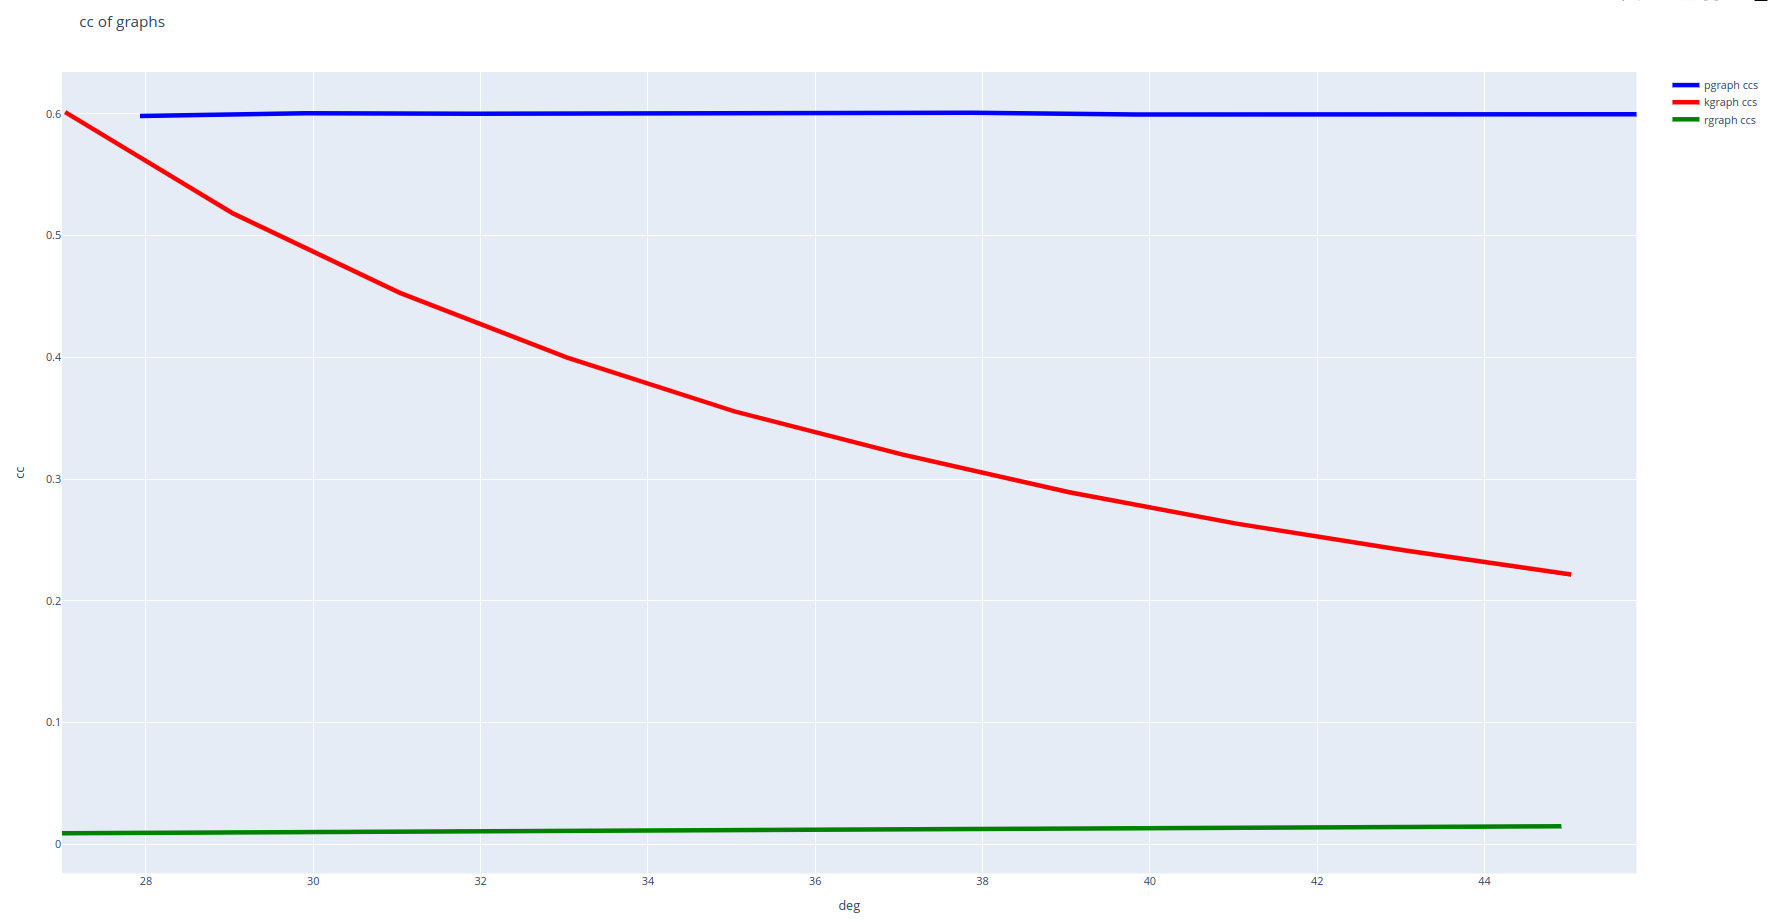
\includegraphics[scale=0.25]{./pictures/cc_better.png}
    \caption{сс от степени вершин} \label{сс}
\end{figure}

Выводы исходя из графика:

\begin{itemize}
    \item граф Пономаренко стабильно дуржит коеффицент класстеризации на уровне 0.6 вне
    зависимости от степени вершины 
    \item граф Клайнберга же равне 0.6 только в начале, когда в нём отсутствуют длинные рёбра.
    После чего, по очевидными причинам, с ростом числа случайных рёбер заметен спад.
    \item Случайный граф Erdos-Renye на протяжении всего промежутка имеет неизменный, очень
    слабо класстеризован
\end{itemize}
Результаты согласуются с теоретическими предположениями

Исходные данные:
\begin{itemize}
    \item для графа Клайнберга были выбраны следующие параметры: Кол-во коротких связей: 10. Кол-во длинных
рёбер варьировалось от 0 до 10
    \item для графа Пономаренко первым параметром(число повторений) было выбрано 8 (Это оптимальное решение,
обоснование будет чуть дальше). Второй параметр варьировался от 15 до 25
    \item В полностью случайном графе можно явно задать степень вершины, она варьирвалась от 20 до 40
\end{itemize}


\subsubsection{Тест на среднюю длину пути}

\subsubsection{Loss тест}

Теперь перейдём к самому главному, точность поиска.
Определять точность будем по следующему принципу: Будем запускать алгоритм 1000 раз и 
суммировать расстояние от найденной вершины, до целевой(выбирается случайно).
Чем меньше будет значение, тем лучше наш алгоритм справляется с поиском ближайшего соседа

Взглянем на график:
\begin{figure}[H]
    \centering
    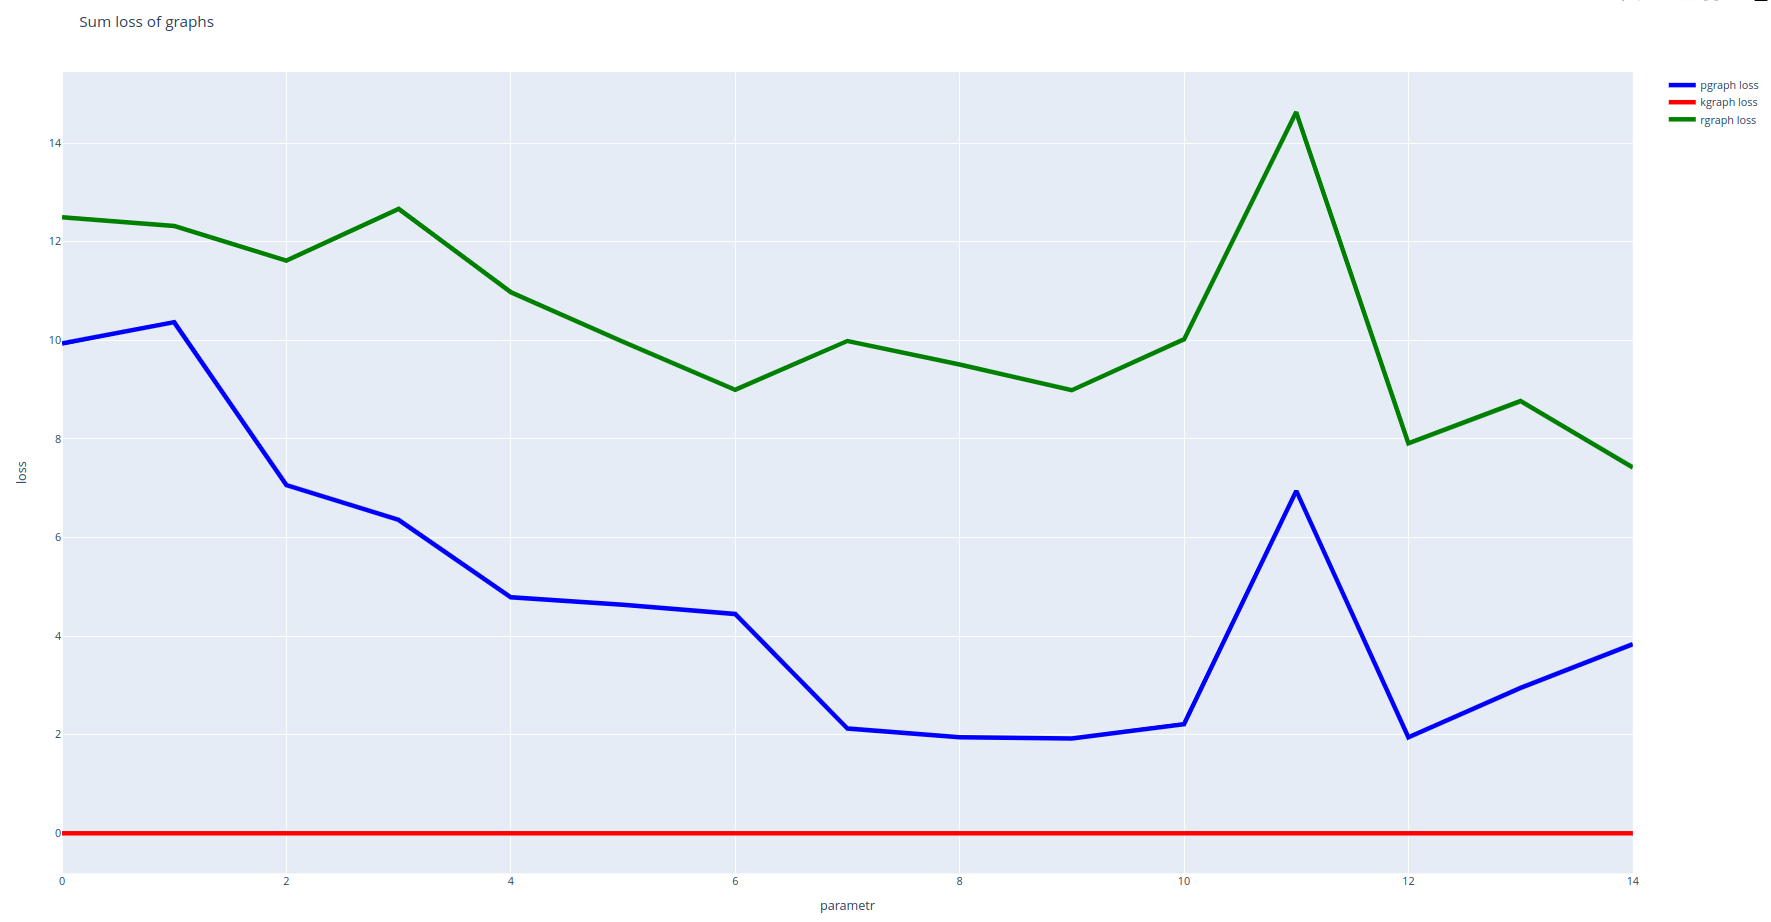
\includegraphics[scale=0.25]{./pictures/sum_loss_imp1.png}
    \caption{Средняя ошибка, параметр "Кол-во повторных поисков" в гарфе Пономаренко = 1 } \label{sum_loss}
\end{figure}


Выводы исходя из графика:

\begin{itemize}
    \item граф Клайнберга показал себя лучше всех, не допустив ни одной ошибки за все 1000 поисков
    \item граф Пономаренко, хоть и работает лучше случайного, но всё ещё стабильно ошибается
\end{itemize}

Теперь рассмотрим только граф Пономаренко и увеличим кол-во поисков:
\begin{figure}[H]
    \centering
    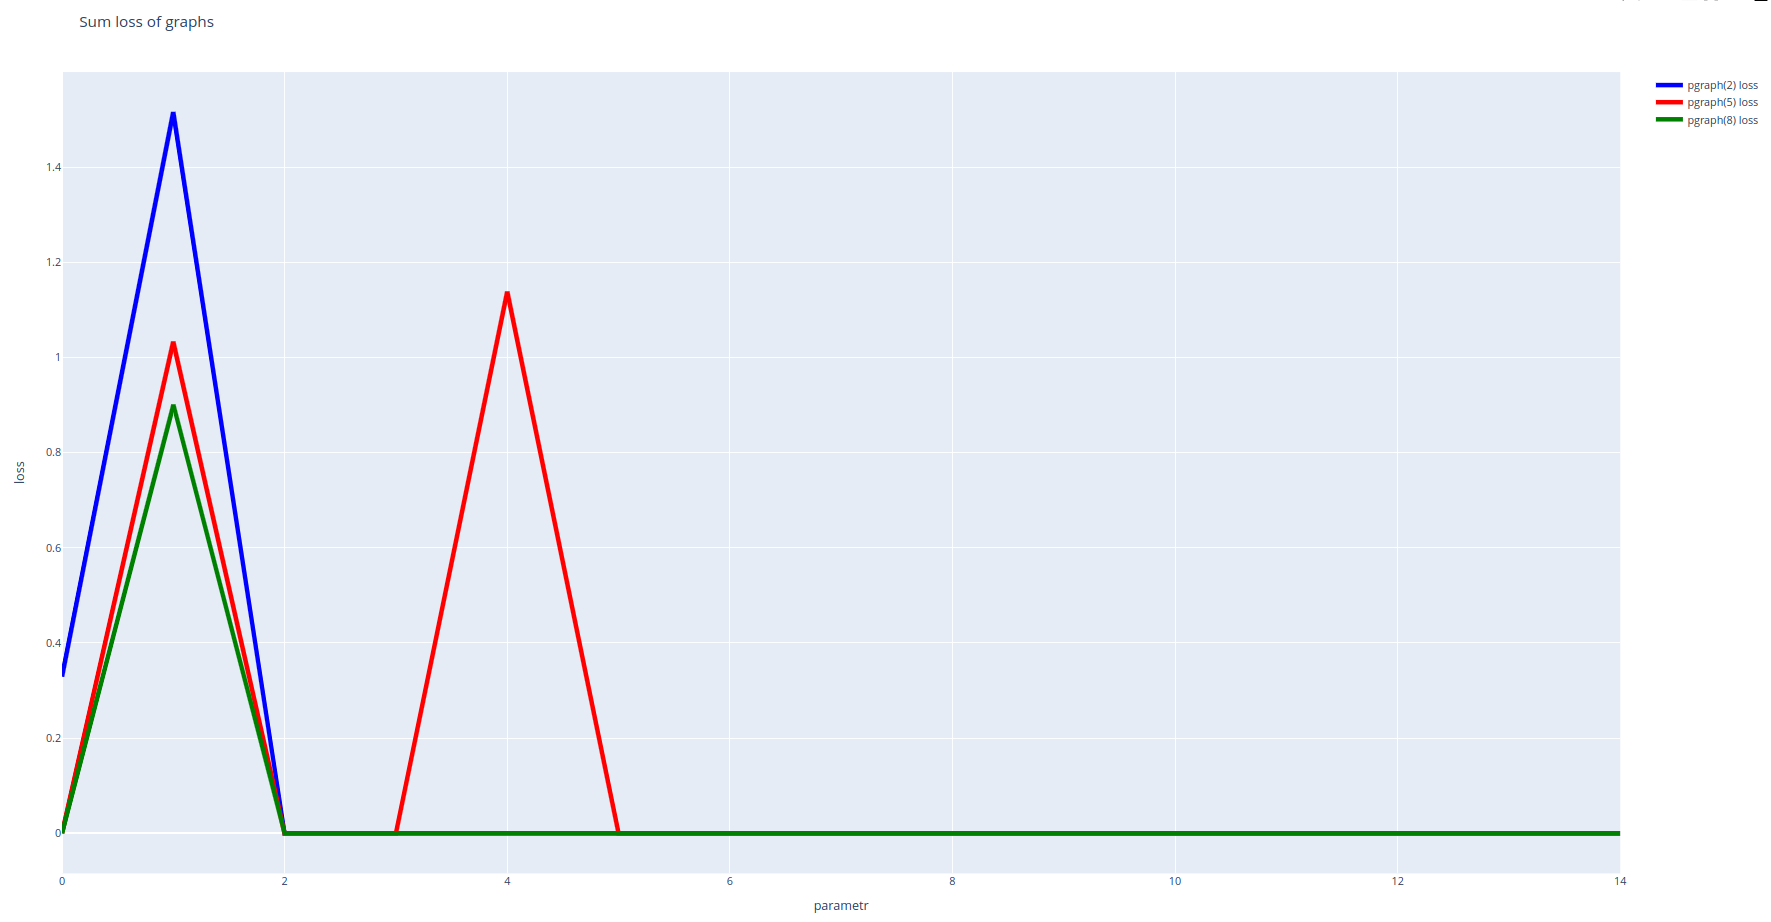
\includegraphics[scale=0.25]{./pictures/sum_loss_Ponomarenko.png}
    \caption{Число поисков 2, 5, 7} \label{sum_loss_Ponomarenko}
\end{figure}

Заметим, что действительно с ростом числа поисков, ошибка по данной метрике становится всё меньше
Из наблюдений Нижегородских математиков достаточное кол-во повторений log(3000) = 8
что согласуется с наблюдениями


